\documentclass[a4paper, 12pt]{report}
\usepackage{graphicx}
\usepackage{amsmath, amsthm, amssymb}
\usepackage{enumerate}
\usepackage{hyperref}
\usepackage{caption}
\usepackage[normalem]{ulem}
\usepackage{pdfpages}
\usepackage[toc,page]{appendix}
\usepackage{minted}

%%% blank footnote
\newcommand\blfootnote[1]{
	\begingroup
	\renewcommand\thefootnote{}\footnote{#1}
	\addtocounter{footnote}{-1}
	\endgroup
}
%%%

%%% prevent hyphenation
\tolerance=1
\emergencystretch=\maxdimen
\hyphenpenalty=10000
\hbadness=10000
%%%

%%% minimize
\DeclareMathOperator*{\minimize}{minimize}
%%%

%%%
\def\N{\mathbb{N}}
\def\Z{\mathbb{Z}}
\def\Q{\mathbb{Q}}
\def\R{\mathbb{R}}
\def\F{\mathbb{F}}

\def\tends{\rightarrow}
\def\into{\rightarrow}
\def\half{\frac{1}{2}}
\def\quarter{\frac{1}{4}}

\newcommand{\set}[1]{\left\{ #1 \right\}}
\newcommand{\norm}[1]{\left\Vert #1 \right\Vert}
\newcommand{\card}[1]{\left\vert #1 \right\vert}
\newcommand{\ceil}[1]{\left\lceil #1 \right\rceil}
\newcommand{\floor}[1]{\left\lfloor #1 \right\rfloor}

\DeclareMathOperator{\dia}{dia}
%%%

\title{Notes\\
\large Machine Learning by Andrew Ng on Coursera}
\author{Sparsh Jain}
\date{\today}

\begin{document}

\maketitle
\tableofcontents
% \listoffigures
% \listoftables

\chapter{Introduction}
\emph{Machine learning} (task, experience, performance) can be classified into
\emph{Supervised} and \emph{Unsupervised} learning.

\section{Supervised Learning}
Supervised learning can be basically classified into \emph{Regression} and
\emph{Classification} problems.

\subsection{Regression Problem}
Regression problems work loosely on continuous range of outputs.

\subsection{Classification Problems}
Classification problems work loosely on discrete range of outputs.

\section{Unsupervised Learning}
An example is \emph{Clustering Problem}.

% \blfootnote{Check \autoref{lecture1} for more details.}
\blfootnote{Check \href{lecture_pdf/Lecture1.pdf}{Lecture1.pdf} for more details.}

\chapter{Linear Regression with One Variable}

\section{Notations}
\begin{align*}
	m                  & = \text{number of training examples}             \\
	x\text{'s}         & = \text{`input' variables / features}            \\
	y\text{'s}         & = \text{`output' variables / `target' variables} \\
	(x, y)             & = \text{single training example}                 \\
	(x^{(i)}, y^{(i)}) & = i^{th} \  \text{example}                       \\
\end{align*}

\section{Supervised Learning}
We have a data set (\emph{Training Set}).

Training Set $\rightarrow$ Learning Algorithm $\rightarrow$ $h$ (\emph{hypothesis},
a function $X \to Y$)

\subsection*{To Represent \texorpdfstring{$h$}{}}
\begin{equation*}
	h_\theta(x) = \theta_0 + \theta_1x
\end{equation*}

\subsection*{Cost}
\begin{equation*}
	\minimize_{\theta_0,\ \theta_1} \frac{1}{2m}\sum_1^m(h_\theta(x) - y)^2
\end{equation*}
\subsubsection*{Cost Function}
Squared Error Cost Function
\begin{equation*}
	J(\theta_0, \theta_1) = \frac{1}{2m}\sum_1^m(h_\theta(x) - y)^2
\end{equation*}
\subsection*{}
\begin{equation*}
	\minimize_{\theta_0,\ \theta_1} J(\theta_0, \theta_1)
\end{equation*}

\section{Gradient Descent}
Finds local optimum:
\begin{enumerate}
	\item Start with some value
	\item Get closer to optimum
\end{enumerate}

\subsection*{Algorithm}
\begin{equation*}
	\theta_j := \theta_j - \alpha\frac{\partial}{\partial\theta_j}J(\theta) \ \forall j
\end{equation*}

where $\alpha$ = learning rate

\subsubsection*{Important!}
Simultaneous Update!
\begin{align*}
	temp_j   & := \theta_j - \alpha\frac{\partial}{\partial\theta_j}J(\theta) \ \forall j \\
	\theta_j & := temp_j \ \forall j
\end{align*}

\section{Gradient Descent for Linear Regression}
Cost function for linear regression is convex!

\emph{Batch Gradient Descent}: Each step of gradient descent uses all training examples.

% \blfootnote{Check \autoref{lecture2} for more details.}
\blfootnote{Check \href{lecture_pdf/Lecture2.pdf}{Lecture2.pdf} for more details.}

\chapter{Linear Algebra}
\section{Matrix}
Rectangular array of numbers:
$$
	\begin{bmatrix}
		1 & 2 & 3 \\
		4 & 5 & 6 \\
	\end{bmatrix}
$$

\paragraph*{Dimension of the matrix:} \#rows x \#cols (2 x 3)

\paragraph*{Elements of the matrix:}
\begin{align*}
	A      & =	\begin{bmatrix}
		1 & 2 & 3 \\
		4 & 5 & 6 \\
	\end{bmatrix}                                \\
	A_{ij} & = \text{``$i,j$ entry'' in the $i^{th}$ row, $j^{th}$ col} \\
\end{align*}

\section{Vector}
An $n \times 1$ matrix.
\begin{align*}
	y & =	\begin{bmatrix}
		1 \\
		2 \\
		3 \\
		4 \\
	\end{bmatrix} \\
	y_i = i^{th} \text{ element}    \\
\end{align*}

\paragraph*{Note:} Uppercase for matrices, lowercase for vectors.

\section{Addition and Scalar Multiplication}
Add/Subtract (element by element) matrices of same dimention only!

Multiply/Divide (all elements) a matrix by scalar!

\section{Matrix Matrix Multiplication}
$m \times n$ matrix multiplied by $n \times o$ matrix gives a $m \times o$ matrix.

\subsection*{Properties}
\begin{enumerate}
	\item Matrix Multiplication is \emph{not} Commutative.
	\item Matrix Multiplication is Associative.
	\item \emph{Identity Matrix ($I$):} $1$'s along diagonal, $0$'s everywhere else in an
	      $n \times n$ matrix. $AI = IA = A$.
\end{enumerate}

\section{Inverse and Transpose}

\subsection*{Inverse}
Only square ($n \times n$) matrices \emph{may} have an inverse.

$$AA^{-1} = A^{-1}A = I$$.

Matrices that don't have an inverse	are \emph{singular} or \emph{degenerate} matrices.

\subsection*{Transpose}
Let $A$ be an $m \times n$ matrix and let $B = A^T$, then
$$ B_{ij} = A_{ji} $$
Example:
\begin{align*}
	A       & =	\begin{bmatrix}
		1 & 2 & 3 \\
		4 & 5 & 6 \\
	\end{bmatrix} \\
	B = A^T & =	\begin{bmatrix}
		1 & 4 \\
		2 & 5 \\
		3 & 6 \\
	\end{bmatrix} \\
\end{align*}

% \blfootnote{Check \autoref{lecture3} for more details.}
\blfootnote{Check \href{lecture_pdf/Lecture3.pdf}{Lecture3.pdf} for more details.}

\chapter{Linear Regression with Multiple Variables}

\section{Notations}
\begin{align*}
	n         & = \text{number of features}                                \\
	x^{(i)}   & = \text{input (features) of $i^{th}$ training example}     \\
	x_j^{(i)} & = \text{value of feature $j$ of $i^{th}$ training example} \\
\end{align*}

\section{Hypothesis}
\subsection*{Previously:}
\begin{equation*}
	h_\theta(x) = \theta_0 + \theta_1x\\
\end{equation*}
\subsection*{Now:}
\begin{equation*}
	h_\theta(x) = \theta_0	+ \theta_1x_1 + \theta_2x_2 + \dots + \theta_nx_n\\
\end{equation*}

For convinience, define $x_0 = 1$. So
\begin{align*}
	h_\theta(x) & = \theta_0x_0	+ \theta_1x_1 + \theta_2x_2 + \dots + \theta_nx_n   \\
	\\
	x           & = \begin{bmatrix}
		x_0    \\
		x_1    \\
		x_2    \\
		\vdots \\
		x_n    \\
	\end{bmatrix} \in \R^{n+1}                      &
	\theta      & = \begin{bmatrix}
		\theta_0 \\
		\theta_1 \\
		\theta_2 \\
		\vdots   \\
		\theta_n \\
	\end{bmatrix} \in \R^{n+1}                        \\
	\\
	h_\theta(x) & = \theta^Tx                                                      \\
\end{align*}

\section{Gradient Descent}

\begin{align*}
	\text{Hypothesis}       & :  h_\theta(x) = \theta^Tx
	                        & = \theta_0x_0 + \theta_1x_1 + \dots + \theta_nx_n              \\
	\text{Parameters}       & : \theta
	                        & =\theta_0, \theta_1, \dots, \theta_n                           \\
	\text{Cost Function}    & : J(\theta) = J(\theta_0, \theta_1, \dots, \theta_n)
	                        & =\frac{1}{2m}\sum_{i=1}^m(h_\theta(x^{(i)}) - y^{(i)})^2       \\
	\text{Gradient Descent} & :                                                              \\
	                        & \text{Repeat} \{                                               \\
	\theta_j                & : =
	\theta_j - \alpha\frac{\partial}{\partial\theta_j}J(\theta)                              \\
	                        & =
	\theta_j - \alpha\frac{\partial}{\partial\theta_j}J(\theta_0, \theta_1, \dots, \theta_n) \\
	                        & =
	\theta_j - \alpha\frac{1}{m}\sum_{i=1}^m(h_\theta(x^{(i)} - y^{(i)})x_j^{(i)})           \\
	\}                      & (\text{simultaneously update }
	\forall j = 0, 1, \dots, n)
\end{align*}

\subsection{Feature Scaling}
\paragraph{Idea:} Make sure features are on a similar scale.

Get every feature into approximately a $-1 \le x_i \le 1$ range.

\subsection{Mean Normalization}
Replace $x_i$ with $x_i - \mu_i$ to make features have approximately zero mean
(Do not apply to $x_0 = 1$).

\subsection*{General Rule}
\begin{equation*}
	x_i \leftarrow \frac{x_i - \mu_i}{S_i}
\end{equation*}
where
\begin{align*}
	\mu_i & = \text{average value of } x_i            \\
	S_i   & = \text{range (max - min)}           & or \\
	      & = \sigma \text{(standard deviation)}
\end{align*}

\subsection{Learning Rate}
$J(\theta)$ should decrease after every iteration. $\#$iterations vary a lot.

Example \emph{Automatic Convergence Test:} Declare convergence if $J(\theta)$
decreases by less than $\epsilon\ (\text{say } 10^{-3})$ in one iteration.

If $J(\theta)$ increases, use smaller $\alpha$. Too small $\alpha$ means slow convergence.

To choose $\alpha$, try $\dots,\ 0.001,\ 0.003,\ 0.01,\ 0.03,\ 0.1,\ 0.3,\ 1,\ \dots$

\section{Features and Polynomial Regression}
\subsection{Features}
Get an insight in your problem and choose better features (may even combine/separate features).

Ex: size = length $\into$ breadth.

\subsection{Polynomial Regression}
Ex: \begin{align*}
	x_1 & = size   \\
	x_2 & = size^2 \\
	x_3 & = size^3 \\
\end{align*}

\section{Normal Equation}
Solve for $\theta$ analytically!
\begin{align*}
	x^{(i)} & = \begin{bmatrix}
		x_0^{(i)} \\
		x_1^{(i)} \\
		\vdots    \\
		x_n^{(i)} \\
	\end{bmatrix} & \in & \ \R^{n+1}            \\
	X       & = \begin{bmatrix}
		(x^{(1)})^T \\
		(x^{(2)})^T \\
		\vdots      \\
		(x^{(m)})^T \\
	\end{bmatrix} & \in & \ \R^{m \times (n+1)} \\
	        & = \begin{bmatrix}
		x_0 & x_1 & \dots & x_n \\
	\end{bmatrix} & \in & \ \R^{m \times (n+1)} \\
	y       & = \begin{bmatrix}
		y^{(1)} \\
		y^{(2)} \\
		\vdots  \\
		y^{(m)} \\
	\end{bmatrix} & \in & \ \R^m                \\
	\theta  & = (X^TX)^{-1}X^Ty                                          \\
\end{align*}

Inverse of a matrix grows as $O(n^3)$, use wisely.

\subsection{Non Invertibility of \texorpdfstring{$X^TX$}{}}
Use 'pinv' function in Octave (pseudo-inverse) instead of 'inv' function (inverse).

If $X^TX$ is non-invertible, common causes are
\begin{enumerate}
	\item Redundant features (linearly dependent)
	\item Too many features ($m \le n$). In this case, delete some features or use \emph{regularization}
\end{enumerate}

\blfootnote{Check \href{lecture_pdf/Lecture4.pdf}{Lecture4.pdf} for more details.}

\chapter{Octave Tutorial}
Check \href{lecture_pdf/Lecture5.pdf}{Lecture5.pdf} for more details.

\chapter{Classification}
Classify into categories (binary or multiple).

\section{Logistic Regression}
\begin{align*}
	0 \le\      & h_\theta(x) \le 1                                               \\
	h_\theta(x) & = g(\theta^Tx)                                                  \\
	g(z)        & = \frac{1}{1 + e^{-z}}        &
	\text{$g$ is called a \emph{sigmoid} function or a \emph{logistic} function.} \\
	h_\theta(x) & = \frac{1}{1 + e^{\theta^Tx}}                                   \\
\end{align*}

\subsection*{Interpretation of Hypothesis Output}
\begin{align*}
	h_\theta(x) & = \text{estimated probability that $y = 1$ on input $x$} \\
	h_\theta(x) & = P(y = 1 | x; \theta) =
	\text{probability that $y = 1$, given $x$, parameterized by $\theta$}  \\
\end{align*}
\begin{equation*}
	P(y = 0 | x; \theta) + P(y = 1 | x; \theta) = 1                  \\
\end{equation*}

\section{Decision Boundary}
\begin{align*}
	\text{Predict: } y & = 1 & \text{ if } h_\theta(x) \ge 0.5         \\
	                   &     & (\theta^Tx \ge 0)                       \\
	\text{Predict: } y & = 0 & \text{ if } h_\theta(x) < 0.5           \\
	                   &     & (\theta^Tx < 0)                         \\
	\theta^Tx          & = 0 & \text{is the \emph{decision boundary.}} \\
\end{align*}

\subsection*{Non-linear Decision Boundaries}
Use same technique as polynomial regression for features.

\section{Cost Function}
\begin{align*}
	\text{Training Set} & :
	\{(x^{(1)}, y^{(1)}), (x^{(2)}, y^{(2)}), ./dots, (x^{(m)}, y^{(m)})\} \\
	x                   & = \begin{bmatrix}
		x_0    \\
		x_1    \\
		\vdots \\
		x_n    \\
	\end{bmatrix} \in \R^{n+1}        \\
	x_0                 & = 1                                              \\
	y                   & \in \{0, 1\}                                     \\
	h_\theta(x)         & = \frac{1}{1 + e^{-\theta^Tx}}                   \\
\end{align*}

\subsection*{How to choose parameter $\theta$?}

\paragraph{Linear Regression:}
\begin{align*}
	J(\theta)                     & =
	\frac{1}{m}\sum_{i = 1}^m\half(h_\theta(x^{(i)}) - y^{(i)})^2      \\
	J(\theta)                     & =
	\frac{1}{m}\sum_{i = 1}^m\mathrm{Cost}(h_\theta(x^{(i)}), y^{(i)}) \\
	\mathrm{Cost}(h_\theta(x), y) & = \half(h_\theta(x) - y)^2         \\
\end{align*}

\paragraph{Logistic Regression:}
\begin{align*}
	\mathrm{Cost}(h_\theta(x), y) & = \begin{cases}
		-\log(h_\theta(x))     & y = 1 \\
		-\log(1 - h_\theta(x)) & y = 0 \\
	\end{cases}    \\
	\mathrm{Cost}(h_\theta(x), y) & = 0 \text{ if } h_\theta(x) = y \\
	\mathrm{Cost}(h_\theta(x), y) &
	\tends \inf \text{ if } y = 0 \text{ and } h_\theta(x) \tends 1 \\
	\mathrm{Cost}(h_\theta(x), y) &
	\tends \inf \text{ if } y = 1 \text{ and } h_\theta(x) \tends 0 \\
\end{align*}

\paragraph{Note:} $y = 0$ or $1$ always.
\begin{align*}
	\mathrm{Cost}(h_\theta(x), y) &
	= -y\log(h_\theta(x)) - (1-y)\log(1 - h_\theta(x))                              \\
	J(\theta)                     &
	= \frac{1}{m}\sum_{i = 1}^m\mathrm{Cost}\left(h_\theta(x^{(i)}), y^{(i)}\right) \\
	                              &
	= -\frac{1}{m}\left[
		\sum_{i=1}^m\left(
		y^{(i)}\log(h_\theta(x^{(i)})) + (1 - y^{(i)})\log(1 - h_\theta(x^{(i)}))
		\right)
		\right]                                                                         \\
\end{align*}

\paragraph{To fit parameters $\theta$:}
\begin{equation*}
	\minimize_\theta J(\theta)
\end{equation*}

\paragraph{To make a prediction given a new $x$:}
\begin{equation*}
	\text{Output } h_\theta(x) = \frac{1}{1 + e^{-\theta^Tx}}
\end{equation*}

\subsubsection{Gradient Descent:}
Simultaneously update all $\theta_j$
\begin{equation*}
	\theta_j := \theta_j - \alpha\frac{\partial}{\partial\theta_j}J(\theta)
\end{equation*}
Plug in the derivative
\begin{equation*}
	\theta_j := \theta_j - \alpha\frac{1}{m}\sum_{i=1}^m\left(
	h_\theta(x^{(i)}) - y^{(i)}
	\right)x_j^{(i)}
\end{equation*}
Don't forget feature scaling!

\section{Advanced Optimization:}
Something better than gradient descent:
\begin{enumerate}
	\item Conjugate Gradient
	\item BFGS
	\item L-BFGS
\end{enumerate}
Advantages:
\begin{enumerate}
	\item No need to manually pick $\alpha$
	\item Often faster than gradient descent
\end{enumerate}
Disadvantages:
\begin{enumerate}
	\item More complex
\end{enumerate}
Use libraries! Beware of bad implementations!

\paragraph{How to use:}
We first need to provide a function that evaluates the following two functions
for a given input value of $\theta$.
\begin{enumerate}
	\item $J(\theta)$
	\item $\frac{\partial}{\partial\theta_j}J(\theta)$
\end{enumerate}

\begin{minted}{octave}
% We can write a single function that can return both of these:
function [jVal, gradient] = costFunction(theta)
	jVal = [...code to compute J(theta)...];
	gradient = [...code to compute derivative of J(theta)...];
end
\end{minted}

Then we can use octave's \emph{fminunc()} optimization algorithm along with the
\emph{optimset()} function that creates an object containing the options we
want to send to \emph{fminunc()}.
\begin{minted}{octave}
options = optimset('GradObj', 'on', 'MaxIter', 100);
initialTheta = zeros(2,1);
	[optTheta, functionVal, exitFlag] = fminunc(@costFunction, 
		initialTheta, options);
\end{minted}

\section{Multi-Class Classification}
\subsection{One vs All}
Build a separate binary classifier $h_\theta^{(i)}(x)$ for each class against all
other classes.
\begin{equation*}
	h\theta^{(i)} = P(y = i | x; \theta)\ \forall i
\end{equation*}
On a new input $x$, to make a prediction, pick the class $i$ that maximizes
$h_\theta^{(i)}(x)$

\blfootnote{Check \href{lecture_pdf/Lecture6.pdf}{Lecture6.pdf} for more details.}

\begin{appendices}
	% \chapter{Lecture 1} \label{lecture1}
	% 
\includepdf[pages=-, width=0.9\textwidth]{lecture_pdf/Lecture1.pdf}
	% \chapter{Lecture 2} \label{lecture2}
	% 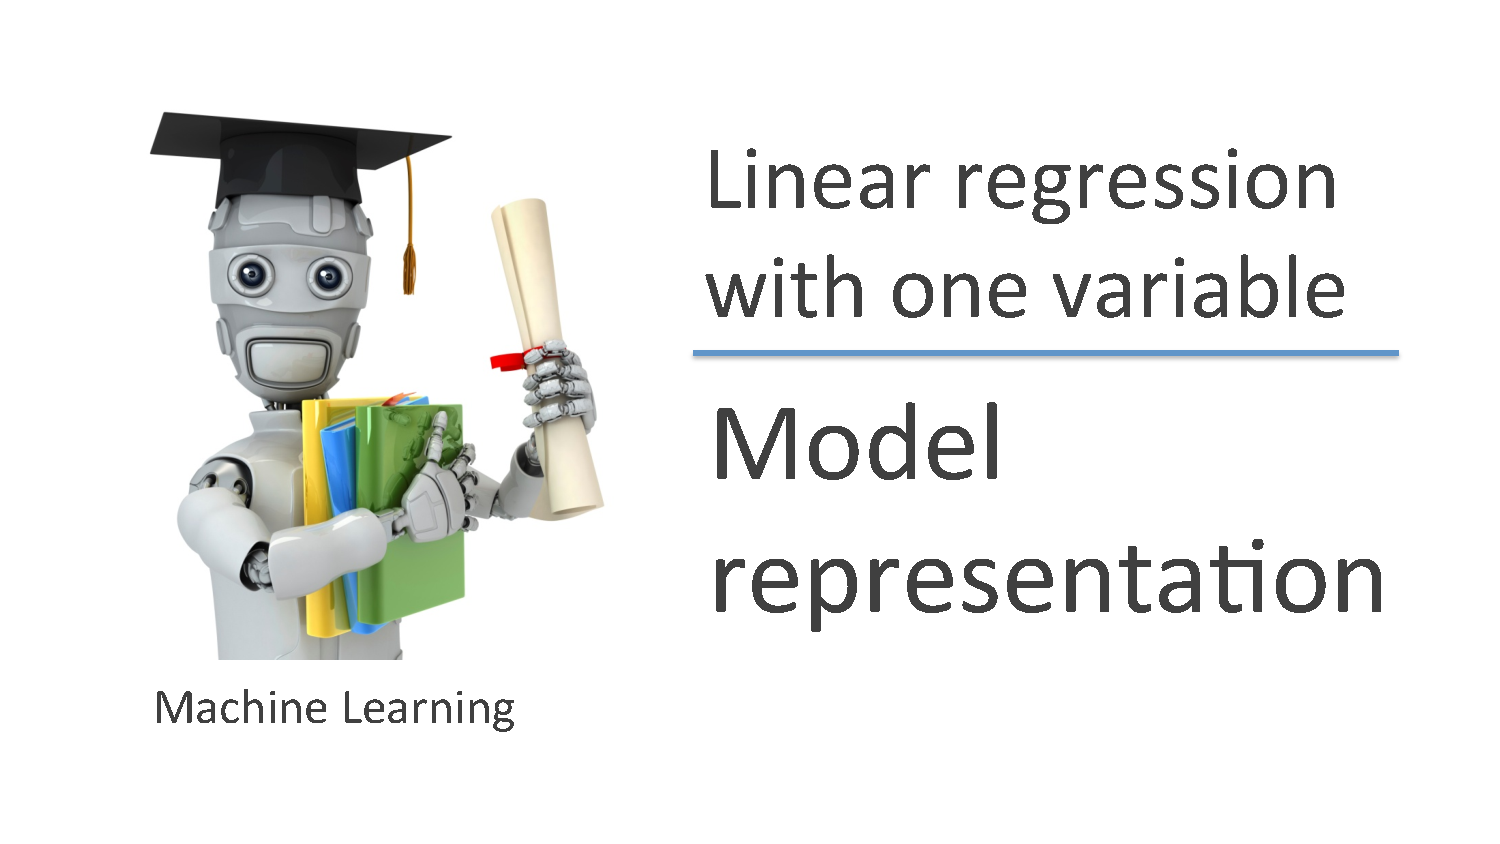
\includepdf[pages=-, width=0.9\textwidth]{lecture_pdf/Lecture2.pdf}
	% \chapter{Lecture 3} \label{lecture3}
	% 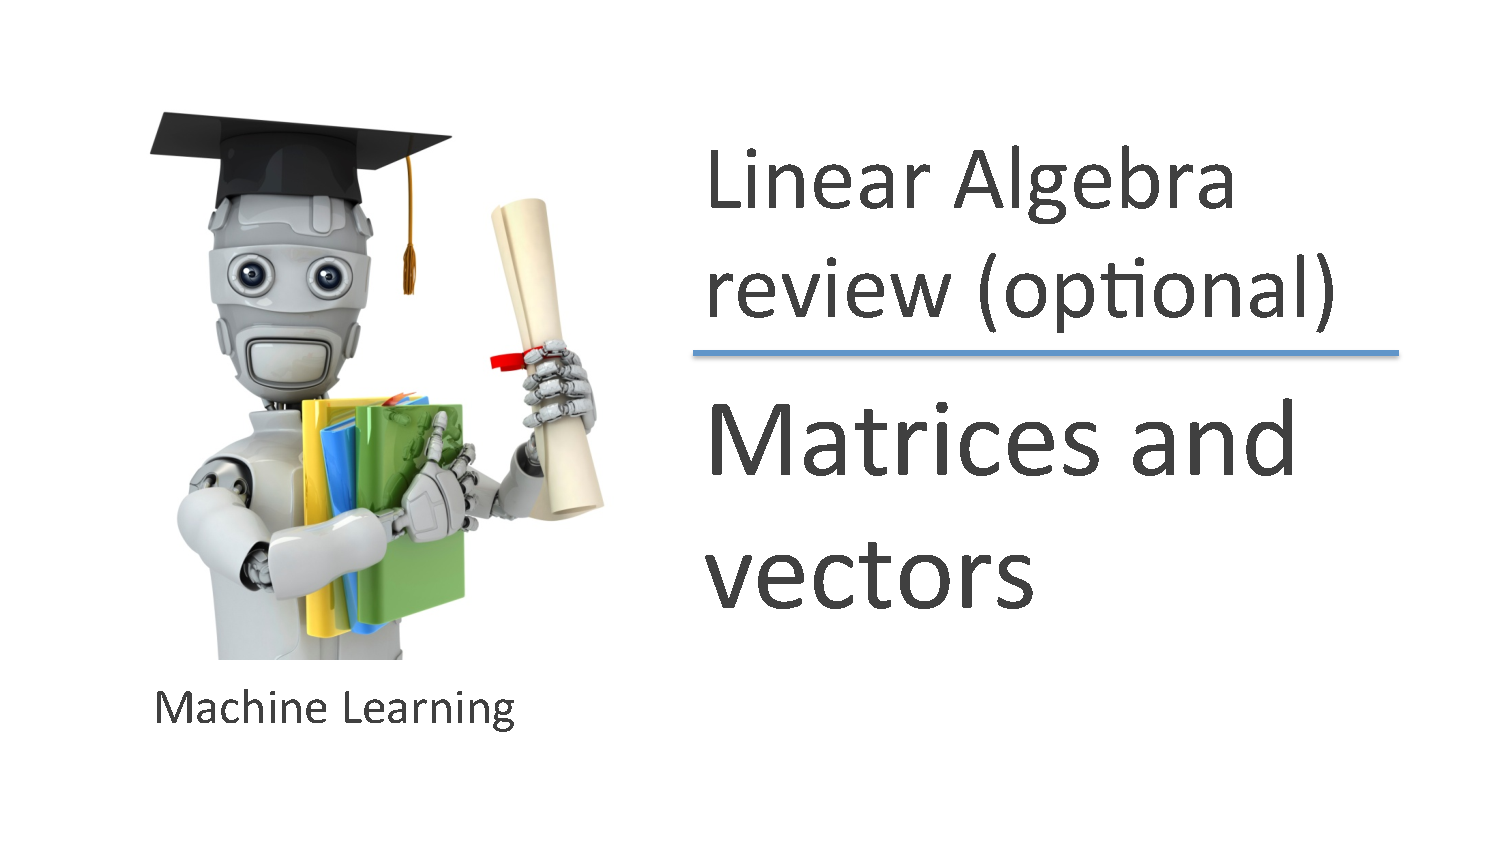
\includepdf[pages=-, width=0.9\textwidth]{lecture_pdf/Lecture3.pdf}
\end{appendices}

\end{document}